% Created by tikzDevice version 0.12.6 on 2026-08-08 02:44:55
% !TEX encoding = UTF-8 Unicode
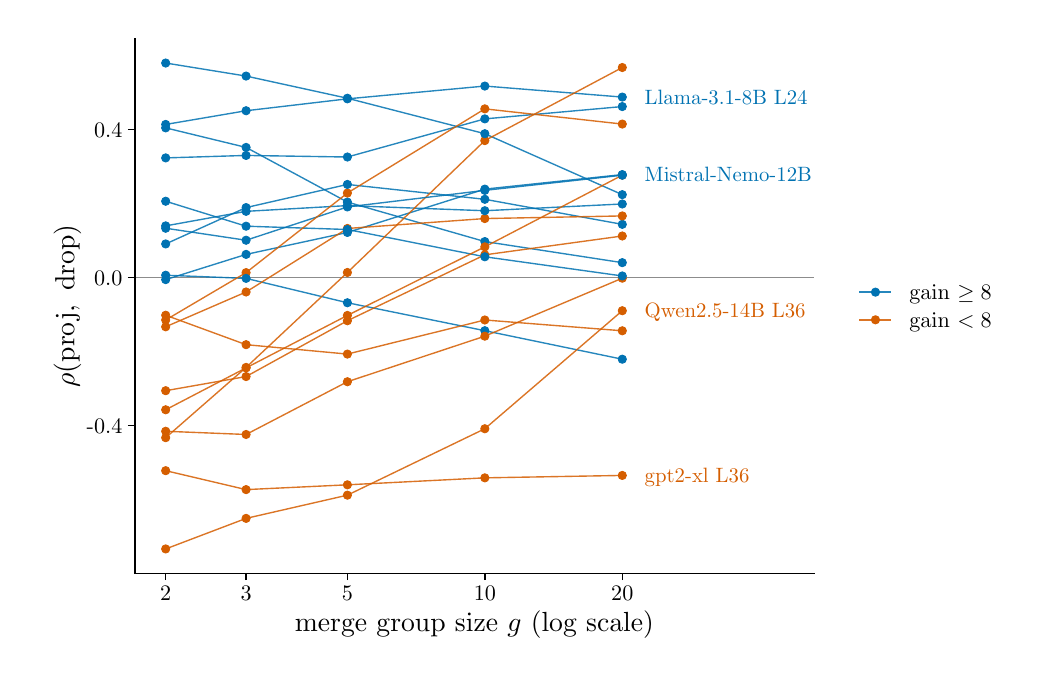
\begin{tikzpicture}[x=1pt,y=1pt]
\definecolor{fillColor}{RGB}{255,255,255}
\path[use as bounding box,fill=fillColor,fill opacity=0.00] (0,0) rectangle (361.35,224.04);
\begin{scope}
\path[clip] (  0.00,  0.00) rectangle (361.35,224.04);
\definecolor{drawColor}{RGB}{255,255,255}
\definecolor{fillColor}{RGB}{255,255,255}

\path[draw=drawColor,line width= 0.5pt,line join=round,line cap=round,fill=fillColor] ( -0.00,  0.00) rectangle (361.35,224.04);
\end{scope}
\begin{scope}
\path[clip] ( 38.72, 26.90) rectangle (284.12,220.04);
\definecolor{fillColor}{RGB}{255,255,255}

\path[fill=fillColor] ( 38.72, 26.90) rectangle (284.12,220.04);
\definecolor{drawColor}{gray}{0.55}

\path[draw=drawColor,line width= 0.3pt,line join=round] ( 38.72,133.81) -- (284.12,133.81);
\definecolor{drawColor}{RGB}{0,114,178}

\path[draw=drawColor,draw opacity=0.85,line width= 0.5pt,line join=round] ( 49.87,134.58) --
	( 78.92,133.45) --
	(115.53,124.64) --
	(165.19,114.54) --
	(214.86,104.24);

\path[draw=drawColor,draw opacity=0.85,line width= 0.5pt,line join=round] ( 49.87,145.89) --
	( 78.92,159.03) --
	(115.53,167.39) --
	(165.19,162.02) --
	(214.86,152.97);

\path[draw=drawColor,draw opacity=0.85,line width= 0.5pt,line join=round] ( 49.87,161.32) --
	( 78.92,152.30) --
	(115.53,151.11) --
	(165.19,141.25) --
	(214.86,134.32);
\definecolor{drawColor}{RGB}{213,94,0}

\path[draw=drawColor,draw opacity=0.85,line width= 0.5pt,line join=round] ( 49.87,120.13) --
	( 78.92,109.49) --
	(115.53,106.09) --
	(165.19,118.41) --
	(214.86,114.51);

\path[draw=drawColor,draw opacity=0.85,line width= 0.5pt,line join=round] ( 49.87, 78.20) --
	( 78.92, 77.04) --
	(115.53, 96.10) --
	(165.19,112.56) --
	(214.86,133.51);

\path[draw=drawColor,draw opacity=0.85,line width= 0.5pt,line join=round] ( 49.87, 63.96) --
	( 78.92, 57.12) --
	(115.53, 58.85) --
	(165.19, 61.37) --
	(214.86, 62.24);
\definecolor{drawColor}{RGB}{0,114,178}

\path[draw=drawColor,draw opacity=0.85,line width= 0.5pt,line join=round] ( 49.87,189.07) --
	( 78.92,194.02) --
	(115.53,198.32) --
	(165.19,202.94) --
	(214.86,198.96);

\path[draw=drawColor,draw opacity=0.85,line width= 0.5pt,line join=round] ( 49.87,187.83) --
	( 78.92,180.77) --
	(115.53,161.02) --
	(165.19,146.75) --
	(214.86,139.13);

\path[draw=drawColor,draw opacity=0.85,line width= 0.5pt,line join=round] ( 49.87,211.26) --
	( 78.92,206.55) --
	(115.53,198.54) --
	(165.19,185.72) --
	(214.86,163.70);

\path[draw=drawColor,draw opacity=0.85,line width= 0.5pt,line join=round] ( 49.87,176.98) --
	( 78.92,177.87) --
	(115.53,177.30) --
	(165.19,191.08) --
	(214.86,195.53);

\path[draw=drawColor,draw opacity=0.85,line width= 0.5pt,line join=round] ( 49.87,133.00) --
	( 78.92,142.11) --
	(115.53,150.04) --
	(165.19,165.70) --
	(214.86,170.95);

\path[draw=drawColor,draw opacity=0.85,line width= 0.5pt,line join=round] ( 49.87,152.42) --
	( 78.92,157.67) --
	(115.53,159.74) --
	(165.19,157.89) --
	(214.86,160.33);
\definecolor{drawColor}{RGB}{213,94,0}

\path[draw=drawColor,draw opacity=0.85,line width= 0.5pt,line join=round] ( 49.87, 75.88) --
	( 78.92,101.27) --
	(115.53,135.58) --
	(165.19,183.23) --
	(214.86,209.64);

\path[draw=drawColor,draw opacity=0.85,line width= 0.5pt,line join=round] ( 49.87, 92.86) --
	( 78.92, 97.97) --
	(115.53,118.14) --
	(165.19,141.95) --
	(214.86,148.76);

\path[draw=drawColor,draw opacity=0.85,line width= 0.5pt,line join=round] ( 49.87, 85.97) --
	( 78.92,101.11) --
	(115.53,120.06) --
	(165.19,144.84) --
	(214.86,170.74);

\path[draw=drawColor,draw opacity=0.85,line width= 0.5pt,line join=round] ( 49.87, 35.68) --
	( 78.92, 46.72) --
	(115.53, 55.11) --
	(165.19, 79.11) --
	(214.86,121.76);
\definecolor{drawColor}{RGB}{0,114,178}

\path[draw=drawColor,draw opacity=0.85,line width= 0.5pt,line join=round] ( 49.87,151.56) --
	( 78.92,147.23) --
	(115.53,159.26) --
	(165.19,165.25) --
	(214.86,170.72);
\definecolor{drawColor}{RGB}{213,94,0}

\path[draw=drawColor,draw opacity=0.85,line width= 0.5pt,line join=round] ( 49.87,118.41) --
	( 78.92,135.53) --
	(115.53,164.28) --
	(165.19,194.70) --
	(214.86,189.21);

\path[draw=drawColor,draw opacity=0.85,line width= 0.5pt,line join=round] ( 49.87,115.95) --
	( 78.92,128.53) --
	(115.53,151.48) --
	(165.19,155.06) --
	(214.86,156.01);
\definecolor{drawColor}{RGB}{213,94,0}
\definecolor{fillColor}{RGB}{213,94,0}

\path[draw=drawColor,line width= 0.3pt,line join=round,line cap=round,fill=fillColor] ( 49.87, 35.68) circle (  1.50);

\path[draw=drawColor,line width= 0.3pt,line join=round,line cap=round,fill=fillColor] ( 78.92, 46.72) circle (  1.50);

\path[draw=drawColor,line width= 0.3pt,line join=round,line cap=round,fill=fillColor] (115.53, 55.11) circle (  1.50);

\path[draw=drawColor,line width= 0.3pt,line join=round,line cap=round,fill=fillColor] (165.19, 79.11) circle (  1.50);

\path[draw=drawColor,line width= 0.3pt,line join=round,line cap=round,fill=fillColor] (214.86,121.76) circle (  1.50);
\definecolor{drawColor}{RGB}{0,114,178}
\definecolor{fillColor}{RGB}{0,114,178}

\path[draw=drawColor,line width= 0.3pt,line join=round,line cap=round,fill=fillColor] ( 49.87,176.98) circle (  1.50);

\path[draw=drawColor,line width= 0.3pt,line join=round,line cap=round,fill=fillColor] ( 78.92,177.87) circle (  1.50);

\path[draw=drawColor,line width= 0.3pt,line join=round,line cap=round,fill=fillColor] (115.53,177.30) circle (  1.50);

\path[draw=drawColor,line width= 0.3pt,line join=round,line cap=round,fill=fillColor] (165.19,191.08) circle (  1.50);

\path[draw=drawColor,line width= 0.3pt,line join=round,line cap=round,fill=fillColor] (214.86,195.53) circle (  1.50);

\path[draw=drawColor,line width= 0.3pt,line join=round,line cap=round,fill=fillColor] ( 49.87,187.83) circle (  1.50);

\path[draw=drawColor,line width= 0.3pt,line join=round,line cap=round,fill=fillColor] ( 78.92,180.77) circle (  1.50);

\path[draw=drawColor,line width= 0.3pt,line join=round,line cap=round,fill=fillColor] (115.53,161.02) circle (  1.50);

\path[draw=drawColor,line width= 0.3pt,line join=round,line cap=round,fill=fillColor] (165.19,146.75) circle (  1.50);

\path[draw=drawColor,line width= 0.3pt,line join=round,line cap=round,fill=fillColor] (214.86,139.13) circle (  1.50);
\definecolor{drawColor}{RGB}{213,94,0}
\definecolor{fillColor}{RGB}{213,94,0}

\path[draw=drawColor,line width= 0.3pt,line join=round,line cap=round,fill=fillColor] ( 49.87, 92.86) circle (  1.50);

\path[draw=drawColor,line width= 0.3pt,line join=round,line cap=round,fill=fillColor] ( 78.92, 97.97) circle (  1.50);

\path[draw=drawColor,line width= 0.3pt,line join=round,line cap=round,fill=fillColor] (115.53,118.14) circle (  1.50);

\path[draw=drawColor,line width= 0.3pt,line join=round,line cap=round,fill=fillColor] (165.19,141.95) circle (  1.50);

\path[draw=drawColor,line width= 0.3pt,line join=round,line cap=round,fill=fillColor] (214.86,148.76) circle (  1.50);

\path[draw=drawColor,line width= 0.3pt,line join=round,line cap=round,fill=fillColor] ( 49.87, 85.97) circle (  1.50);

\path[draw=drawColor,line width= 0.3pt,line join=round,line cap=round,fill=fillColor] ( 78.92,101.11) circle (  1.50);

\path[draw=drawColor,line width= 0.3pt,line join=round,line cap=round,fill=fillColor] (115.53,120.06) circle (  1.50);

\path[draw=drawColor,line width= 0.3pt,line join=round,line cap=round,fill=fillColor] (165.19,144.84) circle (  1.50);

\path[draw=drawColor,line width= 0.3pt,line join=round,line cap=round,fill=fillColor] (214.86,170.74) circle (  1.50);

\path[draw=drawColor,line width= 0.3pt,line join=round,line cap=round,fill=fillColor] ( 49.87, 75.88) circle (  1.50);

\path[draw=drawColor,line width= 0.3pt,line join=round,line cap=round,fill=fillColor] ( 78.92,101.27) circle (  1.50);

\path[draw=drawColor,line width= 0.3pt,line join=round,line cap=round,fill=fillColor] (115.53,135.58) circle (  1.50);

\path[draw=drawColor,line width= 0.3pt,line join=round,line cap=round,fill=fillColor] (165.19,183.23) circle (  1.50);

\path[draw=drawColor,line width= 0.3pt,line join=round,line cap=round,fill=fillColor] (214.86,209.64) circle (  1.50);

\path[draw=drawColor,line width= 0.3pt,line join=round,line cap=round,fill=fillColor] ( 49.87,118.41) circle (  1.50);

\path[draw=drawColor,line width= 0.3pt,line join=round,line cap=round,fill=fillColor] ( 78.92,135.53) circle (  1.50);

\path[draw=drawColor,line width= 0.3pt,line join=round,line cap=round,fill=fillColor] (115.53,164.28) circle (  1.50);

\path[draw=drawColor,line width= 0.3pt,line join=round,line cap=round,fill=fillColor] (165.19,194.70) circle (  1.50);

\path[draw=drawColor,line width= 0.3pt,line join=round,line cap=round,fill=fillColor] (214.86,189.21) circle (  1.50);
\definecolor{drawColor}{RGB}{0,114,178}
\definecolor{fillColor}{RGB}{0,114,178}

\path[draw=drawColor,line width= 0.3pt,line join=round,line cap=round,fill=fillColor] ( 49.87,145.89) circle (  1.50);

\path[draw=drawColor,line width= 0.3pt,line join=round,line cap=round,fill=fillColor] ( 78.92,159.03) circle (  1.50);

\path[draw=drawColor,line width= 0.3pt,line join=round,line cap=round,fill=fillColor] (115.53,167.39) circle (  1.50);

\path[draw=drawColor,line width= 0.3pt,line join=round,line cap=round,fill=fillColor] (165.19,162.02) circle (  1.50);

\path[draw=drawColor,line width= 0.3pt,line join=round,line cap=round,fill=fillColor] (214.86,152.97) circle (  1.50);

\path[draw=drawColor,line width= 0.3pt,line join=round,line cap=round,fill=fillColor] ( 49.87,211.26) circle (  1.50);

\path[draw=drawColor,line width= 0.3pt,line join=round,line cap=round,fill=fillColor] ( 78.92,206.55) circle (  1.50);

\path[draw=drawColor,line width= 0.3pt,line join=round,line cap=round,fill=fillColor] (115.53,198.54) circle (  1.50);

\path[draw=drawColor,line width= 0.3pt,line join=round,line cap=round,fill=fillColor] (165.19,185.72) circle (  1.50);

\path[draw=drawColor,line width= 0.3pt,line join=round,line cap=round,fill=fillColor] (214.86,163.70) circle (  1.50);
\definecolor{drawColor}{RGB}{213,94,0}
\definecolor{fillColor}{RGB}{213,94,0}

\path[draw=drawColor,line width= 0.3pt,line join=round,line cap=round,fill=fillColor] ( 49.87,115.95) circle (  1.50);

\path[draw=drawColor,line width= 0.3pt,line join=round,line cap=round,fill=fillColor] ( 78.92,128.53) circle (  1.50);

\path[draw=drawColor,line width= 0.3pt,line join=round,line cap=round,fill=fillColor] (115.53,151.48) circle (  1.50);

\path[draw=drawColor,line width= 0.3pt,line join=round,line cap=round,fill=fillColor] (165.19,155.06) circle (  1.50);

\path[draw=drawColor,line width= 0.3pt,line join=round,line cap=round,fill=fillColor] (214.86,156.01) circle (  1.50);
\definecolor{drawColor}{RGB}{0,114,178}
\definecolor{fillColor}{RGB}{0,114,178}

\path[draw=drawColor,line width= 0.3pt,line join=round,line cap=round,fill=fillColor] ( 49.87,189.07) circle (  1.50);

\path[draw=drawColor,line width= 0.3pt,line join=round,line cap=round,fill=fillColor] ( 78.92,194.02) circle (  1.50);

\path[draw=drawColor,line width= 0.3pt,line join=round,line cap=round,fill=fillColor] (115.53,198.32) circle (  1.50);

\path[draw=drawColor,line width= 0.3pt,line join=round,line cap=round,fill=fillColor] (165.19,202.94) circle (  1.50);

\path[draw=drawColor,line width= 0.3pt,line join=round,line cap=round,fill=fillColor] (214.86,198.96) circle (  1.50);

\path[draw=drawColor,line width= 0.3pt,line join=round,line cap=round,fill=fillColor] ( 49.87,152.42) circle (  1.50);

\path[draw=drawColor,line width= 0.3pt,line join=round,line cap=round,fill=fillColor] ( 78.92,157.67) circle (  1.50);

\path[draw=drawColor,line width= 0.3pt,line join=round,line cap=round,fill=fillColor] (115.53,159.74) circle (  1.50);

\path[draw=drawColor,line width= 0.3pt,line join=round,line cap=round,fill=fillColor] (165.19,157.89) circle (  1.50);

\path[draw=drawColor,line width= 0.3pt,line join=round,line cap=round,fill=fillColor] (214.86,160.33) circle (  1.50);

\path[draw=drawColor,line width= 0.3pt,line join=round,line cap=round,fill=fillColor] ( 49.87,151.56) circle (  1.50);

\path[draw=drawColor,line width= 0.3pt,line join=round,line cap=round,fill=fillColor] ( 78.92,147.23) circle (  1.50);

\path[draw=drawColor,line width= 0.3pt,line join=round,line cap=round,fill=fillColor] (115.53,159.26) circle (  1.50);

\path[draw=drawColor,line width= 0.3pt,line join=round,line cap=round,fill=fillColor] (165.19,165.25) circle (  1.50);

\path[draw=drawColor,line width= 0.3pt,line join=round,line cap=round,fill=fillColor] (214.86,170.72) circle (  1.50);

\path[draw=drawColor,line width= 0.3pt,line join=round,line cap=round,fill=fillColor] ( 49.87,134.58) circle (  1.50);

\path[draw=drawColor,line width= 0.3pt,line join=round,line cap=round,fill=fillColor] ( 78.92,133.45) circle (  1.50);

\path[draw=drawColor,line width= 0.3pt,line join=round,line cap=round,fill=fillColor] (115.53,124.64) circle (  1.50);

\path[draw=drawColor,line width= 0.3pt,line join=round,line cap=round,fill=fillColor] (165.19,114.54) circle (  1.50);

\path[draw=drawColor,line width= 0.3pt,line join=round,line cap=round,fill=fillColor] (214.86,104.24) circle (  1.50);
\definecolor{drawColor}{RGB}{213,94,0}
\definecolor{fillColor}{RGB}{213,94,0}

\path[draw=drawColor,line width= 0.3pt,line join=round,line cap=round,fill=fillColor] ( 49.87, 63.96) circle (  1.50);

\path[draw=drawColor,line width= 0.3pt,line join=round,line cap=round,fill=fillColor] ( 78.92, 57.12) circle (  1.50);

\path[draw=drawColor,line width= 0.3pt,line join=round,line cap=round,fill=fillColor] (115.53, 58.85) circle (  1.50);

\path[draw=drawColor,line width= 0.3pt,line join=round,line cap=round,fill=fillColor] (165.19, 61.37) circle (  1.50);

\path[draw=drawColor,line width= 0.3pt,line join=round,line cap=round,fill=fillColor] (214.86, 62.24) circle (  1.50);

\path[draw=drawColor,line width= 0.3pt,line join=round,line cap=round,fill=fillColor] ( 49.87, 78.20) circle (  1.50);

\path[draw=drawColor,line width= 0.3pt,line join=round,line cap=round,fill=fillColor] ( 78.92, 77.04) circle (  1.50);

\path[draw=drawColor,line width= 0.3pt,line join=round,line cap=round,fill=fillColor] (115.53, 96.10) circle (  1.50);

\path[draw=drawColor,line width= 0.3pt,line join=round,line cap=round,fill=fillColor] (165.19,112.56) circle (  1.50);

\path[draw=drawColor,line width= 0.3pt,line join=round,line cap=round,fill=fillColor] (214.86,133.51) circle (  1.50);
\definecolor{drawColor}{RGB}{0,114,178}
\definecolor{fillColor}{RGB}{0,114,178}

\path[draw=drawColor,line width= 0.3pt,line join=round,line cap=round,fill=fillColor] ( 49.87,133.00) circle (  1.50);

\path[draw=drawColor,line width= 0.3pt,line join=round,line cap=round,fill=fillColor] ( 78.92,142.11) circle (  1.50);

\path[draw=drawColor,line width= 0.3pt,line join=round,line cap=round,fill=fillColor] (115.53,150.04) circle (  1.50);

\path[draw=drawColor,line width= 0.3pt,line join=round,line cap=round,fill=fillColor] (165.19,165.70) circle (  1.50);

\path[draw=drawColor,line width= 0.3pt,line join=round,line cap=round,fill=fillColor] (214.86,170.95) circle (  1.50);

\path[draw=drawColor,line width= 0.3pt,line join=round,line cap=round,fill=fillColor] ( 49.87,161.32) circle (  1.50);

\path[draw=drawColor,line width= 0.3pt,line join=round,line cap=round,fill=fillColor] ( 78.92,152.30) circle (  1.50);

\path[draw=drawColor,line width= 0.3pt,line join=round,line cap=round,fill=fillColor] (115.53,151.11) circle (  1.50);

\path[draw=drawColor,line width= 0.3pt,line join=round,line cap=round,fill=fillColor] (165.19,141.25) circle (  1.50);

\path[draw=drawColor,line width= 0.3pt,line join=round,line cap=round,fill=fillColor] (214.86,134.32) circle (  1.50);
\definecolor{drawColor}{RGB}{213,94,0}
\definecolor{fillColor}{RGB}{213,94,0}

\path[draw=drawColor,line width= 0.3pt,line join=round,line cap=round,fill=fillColor] ( 49.87,120.13) circle (  1.50);

\path[draw=drawColor,line width= 0.3pt,line join=round,line cap=round,fill=fillColor] ( 78.92,109.49) circle (  1.50);

\path[draw=drawColor,line width= 0.3pt,line join=round,line cap=round,fill=fillColor] (115.53,106.09) circle (  1.50);

\path[draw=drawColor,line width= 0.3pt,line join=round,line cap=round,fill=fillColor] (165.19,118.41) circle (  1.50);

\path[draw=drawColor,line width= 0.3pt,line join=round,line cap=round,fill=fillColor] (214.86,114.51) circle (  1.50);

\node[text=drawColor,anchor=base west,inner sep=0pt, outer sep=0pt, scale=  0.75] at (222.98,119.16) {Qwen2.5-14B L36};
\definecolor{drawColor}{RGB}{0,114,178}

\node[text=drawColor,anchor=base west,inner sep=0pt, outer sep=0pt, scale=  0.75] at (222.98,196.36) {Llama-3.1-8B L24};
\definecolor{drawColor}{RGB}{213,94,0}

\node[text=drawColor,anchor=base west,inner sep=0pt, outer sep=0pt, scale=  0.75] at (222.98, 59.65) {gpt2-xl L36};
\definecolor{drawColor}{RGB}{0,114,178}

\node[text=drawColor,anchor=base west,inner sep=0pt, outer sep=0pt, scale=  0.75] at (222.98,168.35) {Mistral-Nemo-12B L30};
\end{scope}
\begin{scope}
\path[clip] (  0.00,  0.00) rectangle (361.35,224.04);
\definecolor{drawColor}{RGB}{0,0,0}

\path[draw=drawColor,line width= 0.5pt,line join=round,line cap=rect] ( 38.72, 26.90) --
	( 38.72,220.04);
\end{scope}
\begin{scope}
\path[clip] (  0.00,  0.00) rectangle (361.35,224.04);
\definecolor{drawColor}{RGB}{0,0,0}

\node[text=drawColor,anchor=base east,inner sep=0pt, outer sep=0pt, scale=  0.80] at ( 34.22, 77.57) {-0.4};

\node[text=drawColor,anchor=base east,inner sep=0pt, outer sep=0pt, scale=  0.80] at ( 34.22,131.05) {0.0};

\node[text=drawColor,anchor=base east,inner sep=0pt, outer sep=0pt, scale=  0.80] at ( 34.22,184.53) {0.4};
\end{scope}
\begin{scope}
\path[clip] (  0.00,  0.00) rectangle (361.35,224.04);
\definecolor{drawColor}{RGB}{0,0,0}

\path[draw=drawColor,line width= 0.5pt,line join=round] ( 36.22, 80.33) --
	( 38.72, 80.33);

\path[draw=drawColor,line width= 0.5pt,line join=round] ( 36.22,133.81) --
	( 38.72,133.81);

\path[draw=drawColor,line width= 0.5pt,line join=round] ( 36.22,187.28) --
	( 38.72,187.28);
\end{scope}
\begin{scope}
\path[clip] (  0.00,  0.00) rectangle (361.35,224.04);
\definecolor{drawColor}{RGB}{0,0,0}

\path[draw=drawColor,line width= 0.5pt,line join=round,line cap=rect] ( 38.72, 26.90) --
	(284.12, 26.90);
\end{scope}
\begin{scope}
\path[clip] (  0.00,  0.00) rectangle (361.35,224.04);
\definecolor{drawColor}{RGB}{0,0,0}

\path[draw=drawColor,line width= 0.5pt,line join=round] ( 49.87, 24.40) --
	( 49.87, 26.90);

\path[draw=drawColor,line width= 0.5pt,line join=round] ( 78.92, 24.40) --
	( 78.92, 26.90);

\path[draw=drawColor,line width= 0.5pt,line join=round] (115.53, 24.40) --
	(115.53, 26.90);

\path[draw=drawColor,line width= 0.5pt,line join=round] (165.19, 24.40) --
	(165.19, 26.90);

\path[draw=drawColor,line width= 0.5pt,line join=round] (214.86, 24.40) --
	(214.86, 26.90);
\end{scope}
\begin{scope}
\path[clip] (  0.00,  0.00) rectangle (361.35,224.04);
\definecolor{drawColor}{RGB}{0,0,0}

\node[text=drawColor,anchor=base,inner sep=0pt, outer sep=0pt, scale=  0.80] at ( 49.87, 16.89) {2};

\node[text=drawColor,anchor=base,inner sep=0pt, outer sep=0pt, scale=  0.80] at ( 78.92, 16.89) {3};

\node[text=drawColor,anchor=base,inner sep=0pt, outer sep=0pt, scale=  0.80] at (115.53, 16.89) {5};

\node[text=drawColor,anchor=base,inner sep=0pt, outer sep=0pt, scale=  0.80] at (165.19, 16.89) {10};

\node[text=drawColor,anchor=base,inner sep=0pt, outer sep=0pt, scale=  0.80] at (214.86, 16.89) {20};
\end{scope}
\begin{scope}
\path[clip] (  0.00,  0.00) rectangle (361.35,224.04);
\definecolor{drawColor}{RGB}{0,0,0}

\node[text=drawColor,anchor=base,inner sep=0pt, outer sep=0pt, scale=  1.00] at (161.42,  5.94) {merge group size $g$ (log scale)};
\end{scope}
\begin{scope}
\path[clip] (  0.00,  0.00) rectangle (361.35,224.04);
\definecolor{drawColor}{RGB}{0,0,0}

\node[text=drawColor,rotate= 90.00,anchor=base,inner sep=0pt, outer sep=0pt, scale=  1.00] at ( 16.89,123.47) {$\rho(\mathrm{proj},\ \mathrm{drop})$};
\end{scope}
\begin{scope}
\path[clip] (  0.00,  0.00) rectangle (361.35,224.04);
\definecolor{fillColor}{RGB}{255,255,255}

\path[fill=fillColor] (294.12,108.47) rectangle (353.35,138.47);
\end{scope}
\begin{scope}
\path[clip] (  0.00,  0.00) rectangle (361.35,224.04);
\definecolor{fillColor}{RGB}{255,255,255}

\path[fill=fillColor] (299.12,123.47) rectangle (313.58,133.47);
\definecolor{drawColor}{RGB}{0,114,178}

\path[draw=drawColor,draw opacity=0.85,line width= 0.5pt,line join=round] (300.57,128.47) -- (312.13,128.47);
\definecolor{drawColor}{RGB}{0,114,178}
\definecolor{fillColor}{RGB}{0,114,178}

\path[draw=drawColor,line width= 0.3pt,line join=round,line cap=round,fill=fillColor] (306.35,128.47) circle (  1.50);
\end{scope}
\begin{scope}
\path[clip] (  0.00,  0.00) rectangle (361.35,224.04);
\definecolor{fillColor}{RGB}{255,255,255}

\path[fill=fillColor] (299.12,113.47) rectangle (313.58,123.47);
\definecolor{drawColor}{RGB}{213,94,0}

\path[draw=drawColor,draw opacity=0.85,line width= 0.5pt,line join=round] (300.57,118.47) -- (312.13,118.47);
\definecolor{drawColor}{RGB}{213,94,0}
\definecolor{fillColor}{RGB}{213,94,0}

\path[draw=drawColor,line width= 0.3pt,line join=round,line cap=round,fill=fillColor] (306.35,118.47) circle (  1.50);
\end{scope}
\begin{scope}
\path[clip] (  0.00,  0.00) rectangle (361.35,224.04);
\definecolor{drawColor}{RGB}{0,0,0}

\node[text=drawColor,anchor=base west,inner sep=0pt, outer sep=0pt, scale=  0.80] at (318.58,125.71) {gain $\geq 8$};
\end{scope}
\begin{scope}
\path[clip] (  0.00,  0.00) rectangle (361.35,224.04);
\definecolor{drawColor}{RGB}{0,0,0}

\node[text=drawColor,anchor=base west,inner sep=0pt, outer sep=0pt, scale=  0.80] at (318.58,115.71) {gain $< 8$};
\end{scope}
\end{tikzpicture}
